\section{Time Performance}\label{sec:time-performance}
In addition to experiments measuring the performance of our system, we also wanted to test its retrieval speed.
The speed was measured in two different scenarios.
In the first scenario, we do not insert any query, thus making the system send a non-KNN query to Elastic (Section~\ref{sec:dsl-compiler}).
In the second case, we insert a random three-word query (words were generated by an API \footnote{https://random-word-api.herokuapp.com/
}) for each iteration of the experiment.
In addition, in both scenarios, we ran each step 10 times, and with this data, we also computed the standard error for each step.\\ \\
The experiment was run for both scenarios for 12 different values of $K$ -- from 10 to 120 with a step of 10 documents.
Each time, we increased the size of the returned page by 10.
In the case of the first scenario, only the \verb|size| parameter was modified -- since it's not a KNN query.
On the other hand, when running the tests for the second scenario, we also increased the value of the \verb|k| parameter for each step.
Moreover, in the case of the second scenario, for each of the ten repetitions of a step, we generated -- as we said previously -- three words to be used as a query for the approximate KNN search.
This was done in order to try and force Elasticsearch to always perform a search from scratch, not using any cached data from previous search queries. \\ \\
For each scenario, we compute the retrieval time for each combination of fields.
Since we can filter for the \verb|metadata| and \verb|specification| fields, we tested the times for only metadata, only specification, and both metadata and specification.
The obtained graph can be seen in Figure~\ref{fig:time}.
Tables~\ref{tab:times-no-queries} and~\ref{tab:times-queries} display all the mean retrieval times -- in milliseconds -- at each $@K$ for the \("\)no queries\("\) and \("\)random queries\("\) experiments.
From the two graphs, we can see that in the case of the \("\)no queries\("\) experiment, the retrieval times seem to plateau when we go over 90 documents per page.
On the other side, in the \("\)random queries\("\), we see more of a linear increase in retrieval times as $K$ increases.

\begin{figure}[!h]
    \begin{center}
        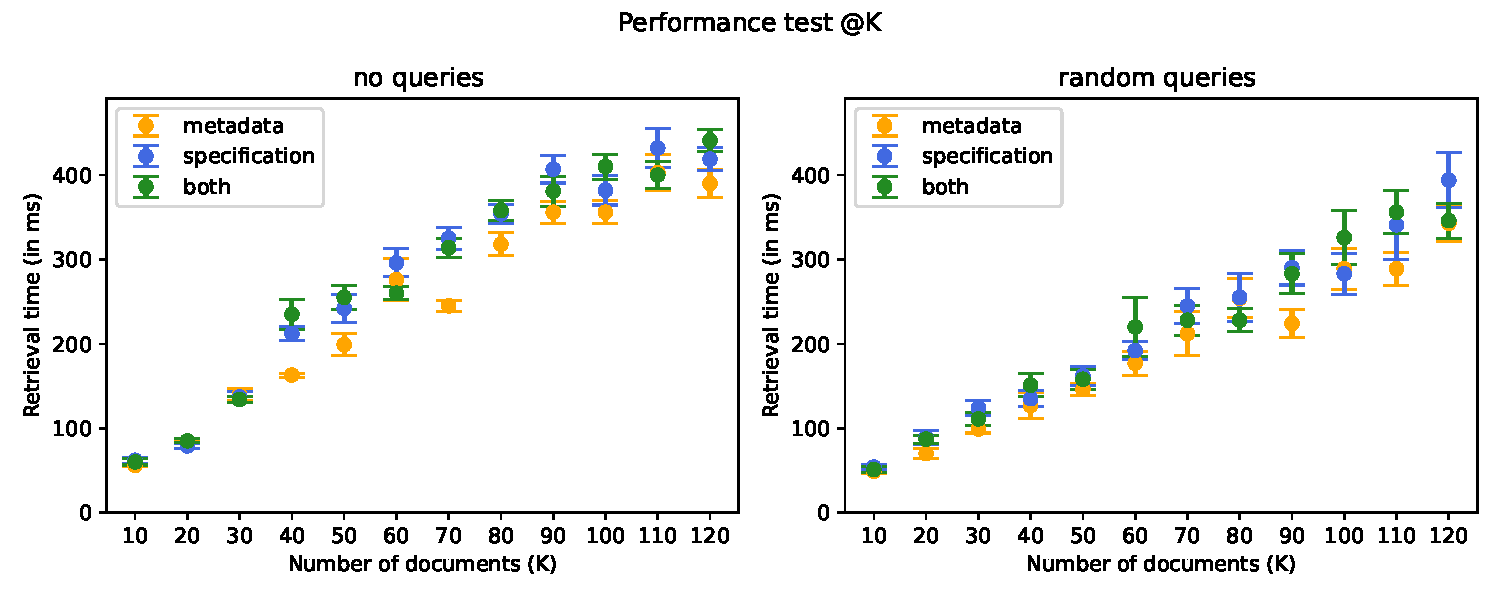
\includegraphics[width=0.8\linewidth]{assets/pdf/evaluation/time}
    \end{center}

    \caption{Retrieval times in milliseconds. Bars indicate the standard error}
    \label{fig:time}
\end{figure}

\begin{table}[!h]
    \begin{center}
        \begin{tabular}{l c c c c c c c c c c c c}
            \hline
            \textbf{Field} & \textbf{@10} & \textbf{@20} & \textbf{@30} & \textbf{@40} & \textbf{@50} & \textbf{@60} & \textbf{@70} & \textbf{@80} & \textbf{@90} & \textbf{@100} & \textbf{@110} & \textbf{@120} \\ \hline
            Metadata & 56 & 80 & 140 & 163 & 199 & 276 & 245 & 318 & 356 & 356 & 403 & 390 \\
            Specification & 62 & 79 & 137 & 212 & 242 & 296 & 325 & 354 & 407 & 382 & 432 & 419 \\
            Both & 60 & 85 & 134 & 235 & 255 & 260 & 314 & 358 & 381 & 410 & 400 & 441 \\ \hline \hline
            Mean & 59.3 & 81.3 & 137 & 203.3 & 232 & 277.3 & 294.6 & 343.3 & 381.3 & 382.6 & 411.6 & 416.6 \\ \hline
        \end{tabular}
    \end{center}

    \caption{Retrieval times in milliseconds for the "no queries" experiment}
    \label{tab:times-no-queries}
\end{table}

\begin{table}[!h]
    \begin{center}
        \begin{tabular}{l c c c c c c c c c c c c}
            \hline
            \textbf{Field} & \textbf{@10} & \textbf{@20} & \textbf{@30} & \textbf{@40} & \textbf{@50} & \textbf{@60} & \textbf{@70} & \textbf{@80} & \textbf{@90} & \textbf{@100} & \textbf{@110} & \textbf{@120} \\ \hline
            Metadata & 49 & 70 & 99 & 127 & 146 & 177 & 212 & 254 & 224 & 289 & 289 & 343 \\
            Specification & 54 & 89 & 124 & 135 & 162 & 192 & 245 & 255 & 290 & 283 & 341 & 394 \\
            Both & 51 & 87 & 111 & 151 & 158 & 220 & 228 & 228 & 283 & 326 & 356 & 346 \\ \hline \hline
            Mean & 51.3 & 82.0 & 111.3 & 137.6 & 155.3 & 196.3 & 228.3 & 245.6 & 265.6 & 299.3 & 328.6 & 361 \\ \hline
        \end{tabular}
    \end{center}

    \caption{Mean retrieval times in milliseconds for the "random queries" experiment}
    \label{tab:times-queries}
\end{table}

\noindent Let's now create a causal graph for this batch of experiments.
The graph will be composed of several nodes: \("\)Only Metadata\("\), \("\)Only Specification\("\), \("\)Both\("\), \("\)Random Queries\("\), \("\)No Queries\("\) and \("\)Faster Fetch Time\("\).
The \("\)Only Metadata\("\), \("\)Only Specification\("\), and \("\)Both\("\) nodes means that we only take into account the retrieval times of queries containing those fields.
The \("\)Random Queries\("\) and \("\)No Queries\("\) nodes mean that we only take into account the mean retrieval times of the queries in one experiment or the other.
Finally, the \("\)Faster Fetch Time\("\) nodes means that the mean retrieval time $@K$ coming from one node is lower than the retrieval time $@K$ coming from their alternative(s).
To clarify this last point, let's take into account the path Only Metadata $\rightarrow$ Faster Fetch Time.
In this case, we have a faster fetch time if the mean coming from the \("\)Only Metadata\("\) node is lower than both the \("\)Only Specification\("\) and \("\)Both\("\) means (that are found in Tables~\ref{tab:times-no-queries} and~\ref{tab:times-queries}). \\ \\
Now, we compute the probabilities for all paths.
For the paths Only Metadata $\rightarrow$ Faster Fetch Time, Only Specification $\rightarrow$ Faster Fetch Time, and Both $\rightarrow$ Faster Fetch Time the probabilities will be:
\[P_1 = \frac{19}{24} = 0.8~~~~~~~~~~~~~~~P_2 = \frac{2}{24} = 0.1~~~~~~~~~~~~~~~P_3 = \frac{3}{24} = 0.1\]
While the probability for the paths Random Queries $\rightarrow$ Faster Fetch Time and No Queries $\rightarrow$ Faster Fetch Time will be:
\[P_4 = \frac{11}{12} = 0.9~~~~~~~~~~~~~~~P_5 = \frac{1}{12} = 0.1\]
The causal graphs are displayed in Figures~\ref{fig:dag-tmp-metadata} and~\ref{fig:dag-tmp-random}.
The final causal graph can be found in Figure~\ref{fig:dag-retrieval}.
This shows that there is a very high probability that, if we either filter for metadata or perform a search request using a query, we will have faster retrieval times.

\begin{figure}[!h]
    \begin{minipage}{0.48\textwidth}
        \centering
        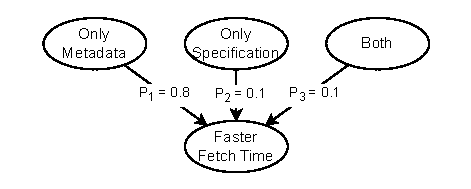
\includegraphics[width=0.9\linewidth]{assets/pdf/evaluation/dag-tmp-meta}
        \caption{Causal graph with probabilities}
        \label{fig:dag-tmp-metadata}
    \end{minipage}\hfill
    \begin{minipage}{0.48\textwidth}
        \centering
        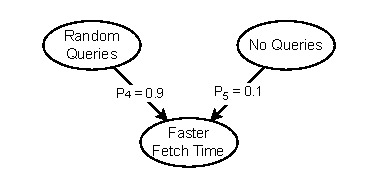
\includegraphics[width=0.8\linewidth]{assets/pdf/evaluation/dag-tmp-random}
        \caption{Causal graph with probabilities}
        \label{fig:dag-tmp-random}
    \end{minipage}

    \label{fig:dag-comparison}
\end{figure}

\begin{figure}[!h]
    \begin{center}
        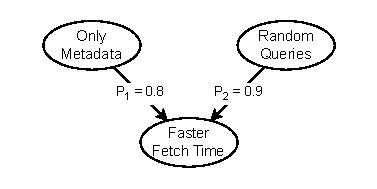
\includegraphics[width=0.4\linewidth]{assets/pdf/evaluation/dag-retrieval}
    \end{center}

    \caption{Causal graph with probabilities}
    \label{fig:dag-retrieval}
\end{figure}
